\documentclass{template/csfourzero}

\usepackage[sort&compress]{natbib}
%\usepackage[sorting=none]{biblatex}
\usepackage{url}
\usepackage{graphicx}
\usepackage{caption}
\usepackage{float}

\bibliographystyle{unsrt}
%\bibliography{myrefs}

\title{An Attempt to illustrate bad Partitioning on a One Node Apache Cassandra System}
\author{Sonke Wohler}
\date{\today}



\begin{document}
\maketitle

\section{Abstract} % 100 words

The NoSQL Database Cassandra is specifically designed to work as a distributed Database by the use of partitions. These are usually used to evenly distribute Data within a distributed Cluster of Servers when used correctly, but there is thus far no significant literature on the effects of partitioning on a single machine. The assumption is that the same principles will hold for a single Server Database which is to be investigated in this small experiment.


\section{Introduction} % 250 words
\label{sec:intro}

  In the Age of Information, as some call the recent decades, Data has moved to the centre stage in near every Industry, with a resurgence of Artificial Intelligence only accelerating this trend further. With Amazon, Facebook, Google and co as the prime examples, the storage of Data is an integral part of our everyday lives now. \cite{riseNoSQL}
  \\
  With ever increasing demands to the Databases facilitating these services several developments have helped tackle the issues arising from such Database applications. One of these issues is the ability to maintain large Datasets that may be accessed in many places at once. Apache-Cassandra is a distributed NoSQL Database System designed with this in mind.\cite{apacheCassandra,nonsenSQL,amazonFuture}
  \subsection{Cassandra in Principle}
  NoSQL (Not Only SQL) is an adaptation from SQL for non-relational Databases. Non-relational Databases have existed since the 1960s, but have recently seen much use with their ability to scale horizontally; that is to adapt the number of servers or "Nodes" that are used to handle the maintenance of Data to the load placed on the system. By abandoning some of the relational principles of SQL, NoSQL Databases, like Cassandra, can more easily add new Servers and handle large read and write throughput in a distributed manner, while trading in some of its abilities to relate Data, in particular by loosing the ability to perform Joins.\cite{apacheCassandra,nonsenSQL,amazonFuture,cassandraBasics}

\section{Background} % 500 words
\label{sec:lit}

  \subsection{What is Partitioning?}
  In a Distributed Database perhaps the core issue is to know what Nodes to access in an attempt to retrieve Data. Cassandra achieves this by partitioning its Data. Each Partition is assigned to one or more Nodes, depending on the assigned replication factor. Higher replication allows the System to distribute load across several Nodes while increasing the maintenance required to guarantee eventual consistency. A good replication balance is one of the basic optimisation factors for a Cassandra Cluster. \cite{cassandraBasics}
  Data is assigned to a partition by its partition key, which is an integral part of the primary key in Cassandra. Without a partition key Data cannot be retrieved in the first place, in order to prevent heavy load queries that could potentially search the entire Cluster. This is why Joins are not supported.\cite{cassandraKey}
  As such retrieving Data involves two stages, first the partition key identifies the correct Node, then the request is referred to that Node which retrieves the Data from within that Partition. \cite{cassandraRead}
  However, there is nothing to stop one from using Cassandra not as a distributed system but simply on one machine. In this case partitioning is largely superfluous. 
  
  \subsection{Related Work}
  As Cassandra is a distributed System there is little sense in limiting it to one machine and no significant literature can be found on this subject.
  \\
  Analysis of Cassandra performance for the most part is in agreement with stated design goals that writing performance is extremely high, while reading performance is more sensitive. \cite{cassandraBasics,ctoAnalysis} As such it appears reasonable to focus investigations of performance on reading operations before all others. 
  \\
  Both the design of Cassandra and the literature suggest that reading performance will suffer when large partitions are used even when these still spread Data evenly across the Cluster, while spreading the same Data across several partitions will improve performance. \cite{sherman,ctoAnalysis}
  \\
  Lastly all authors so far agree that smaller partitions benefit a Cassandra Cluster by spreading Data more evenly, and that this is the most significant factor in reading performance. \cite{casLimits,cassandraBenchmarks,ctoAnalysis,sherman,cassandraBasics}
  


\section{Research question} % 500 words
\label{sec:rq}
  
  \subsection{The Intend}
  While Partitioning is designed to facilitate distributed systems, it ultimately is a means to group Data. As such there might be an effect on Data retrieval times even when all partitions reside on only one Node. Such a one Node Cluster is not what Cassandra is intended for, but there is currently no literature to suggest that this would have any adverse effects on the efficiency.
  \\
  Design Guidelines for Cassandra generally suggest spreading Data evenly over the Cluster of Nodes.\cite{cassandraBasics,sherman} This usually means to make sure that the rows written to the Database will be distributed evenly to all partitions, which will in turn be assigned evenly to the various Nodes. The ideal case would hence be to have as many partitions as possible, to the point that in extreme cases each entry could be assigned to its own partition. \cite{cassandraBasics} However, even assigning all entries to the same partition would evenly spread Data across a one Node cluster, which begs the question whether there will be any difference in performance based on the way Data is partitioned.
  \\
  As Partitions are used to group Data to the end of locating said Data, and since even within the same machine the exact entry has to be localised perhaps partitioning would still positively affect performance. The partition key is heavily involved in finding the correct SSTable on Disc, unrelated to identifying the correct Node within the Cluster. \cite{cassandraRead} In addition to this smaller partitions would be created which would be searched faster, hence a 'good' partitioning scheme should equally improve reading on one Node. 
  \\
  \subsection{The Hypothesis}
  Reading times for evenly partitioned Data sets should be shorter than for unpartitioned sets. This Hypothesis will have to be tested against the idea that there is no significant difference between the sets' reading times, as it is unlikely that the opposite is the case.
  
  \subsection{Considerations Regarding the Hypothesis}
  Considering the scale of this exercise only very minimal tests can be performed on a small set up. There are many interpretations of good performance and different application require a focus on different quantities. \cite{benchmarkIntro,crud} Minimal tests here mean that only the time between the querying of the DB and the return of the Data is investigated while minimising all other possible influences, rather than including these in the experimental design and investigating the reading time for a variety of conditions, in particular hardware conditions.
  \\ Due to these limitations there is the very real possibility that any effects relating to the hypothesis are too small to be observed.

\section{Experimental Design} % 500 words
\label{sec:exp}
  The quite obvious Idea of this experiment is to set up a single Cassandra Node \cite{apacheCassandra}, to populate this empty DB with entries according to different partitioning schema and to query this Data while recording the time between request and Data return. At least two schema representing a 'good' and a 'bad' way of partitioning Data must be represented, that would spread Data evenly and unevenly across the partitions, respectively. Before and between any tests the DB is cleared of any content to guarantee only the intended Data will have any influence on the experiment.
  \\
  \\
  Only one table was contained in the DB named "customer", with a name and address field representing some arbitrary other data stored in the table. A "cID" integer field was used as a primary clustering key, while the partition key was another "hashID" integer field. Hashing of clustering keys is a reasonable way to control Data partitioning in Cassandra Modelling. \cite{sherman}
  
  \subsection{Data Generation}
  As a 'good' partitioning scheme the partition key was chosen as cID divided by 10 and rounded down to the nearest integer, which creates partitions of exactly 10 entries and perfectly spreads the Data. This scheme was throughout the experiment referred to as the ideal case.
  The opposite schema was to assign all entries to the same partition with hashID=0, which was referred to as the worst case.
  \\
  \\
  For completeness a third schema was chosen that would imitate a Gaussian Distribution of entries across the partitions. The Gaussian would have a standard deviation of 5 and be centred at 0, while the closest integer to its magnitude value would be chosen as the partition key. This schema was intended to imitate common partition issues when some component of the Data is chosen as the partition key, as the Central Limit Theorem dictates that such partition keys will likely follow a standard distribution which would have an impact on the spreading of Data. \cite{centLimit} Hence this schema was referred to as the 'normal' case. 
  \\
  \\
  These Cases were tested by clearing the DB before beginning a counter and creating the entries in accordance with the schema to be tested with cID simply being the current counter state. The counter ended first at 100 entries, and would in subsequent tests increase by a factor of 10 up to 1,000,000. Up to 100,000 entries these tests were performed three times for each case, but due to the time involved in generating the Data the 1,000,000 test was only performed once per schema.
  \\
  \\
  While creating the entries a subset of keys were recorded in an external text file for querying later, first 100 keys and in the 1,000,000 tests 10,000. After populating the DB the System Resources were specifically inspected to ensure consistent conditions in each test. All other machine activities where possible were halted and the internet connection severed to minimise the effect of other processes and the associated noise.
  \\
  The recorded keys were queried in order, with the system time before and after the query request being recorded.
  \subsection{The System and Further Considerations}
  The Apache Cassandra \cite{apacheCassandra} version used was 3.11.3, and set up on machine with largely default configuration. The only exception to this is that key caching was disabled to eliminate its possible effect on the experiment.
  \\
  The Data was generated in a Java program run in jre 1.8.0\_171 from Eclipse IDE and is available on GitHub. \cite{myGit}
  \\
  The Java Program and Cassandra DB were interfaced using the Datastax Java Driver Version 3.5.0, retrieved using Maven 3.5.3. \cite{gitDriver}
  \\
  The keyspace used (named "cs4040") specified a replication factor of 1 to allow running with one Node, and used the "SimpleStrategy" compaction.
  \\
  The Operating System was Microsoft Windows Enterprise Version 10.0.16299 on a HP ZBook 17 G4. \cite{workstation}
  \\
  All further specifications were default and where appropriate automatically amended to default by the System.


\section{Results} % 500 words
\label{sec:results}

  \subsection{The 'Ideal' Case}
  
  Regression, F-Test and t-Test null hypotheses were considered rejected at the 5\% margin.
  
  \begin{figure}[H]
      \centering
      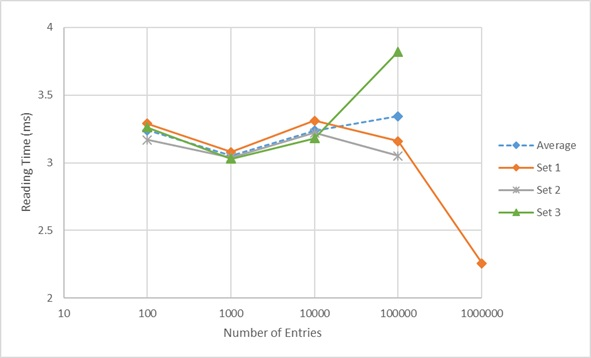
\includegraphics{figures/idealTimes.jpg}
      \caption{Reading Times of 'ideal' partitioning schema for different Number of DB Entries. Measruements for a particular Number of entries were performed three times except for 1,000,000 entries, with average displayed.
      \\
      Regression on Average: r=0.71}
      \label{fig:idealTimes}
  \end{figure}
  
  \begin{figure}[H]
      \centering
      \noindent\makebox[\textwidth]{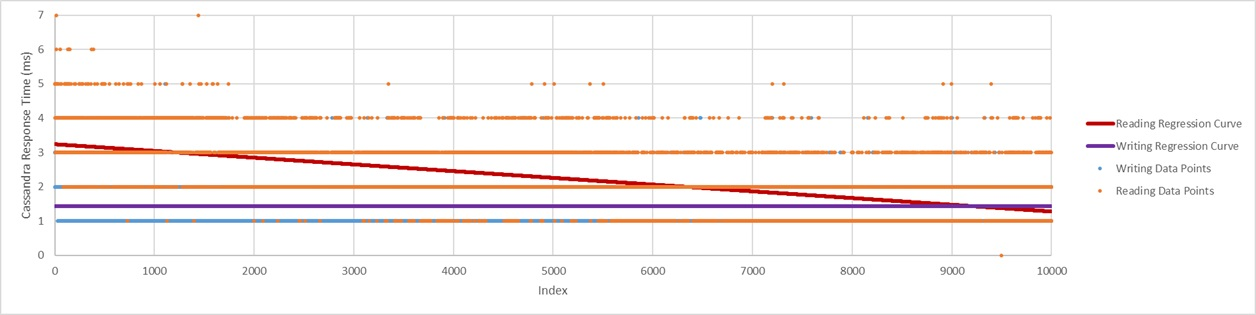
\includegraphics[width=\paperwidth]{figures/idealFull.jpg}}
      \caption{Writing and Reading Times for the 'ideal' partitioning schema, at an Entry Number of 1,000,000 and sample size of 10,000. Note that some outliers above 7 ms (approaching 16 ms) were excluded in the chart in favour of more clear display.
      \\
      Regression: r= 0.009 for writing and r= 0.58 for reading
      }
      \label{fig:idealFull}
  \end{figure}
  
  \subsection{The 'Normal' Case}
  
    \begin{figure}[H]
      \centering
      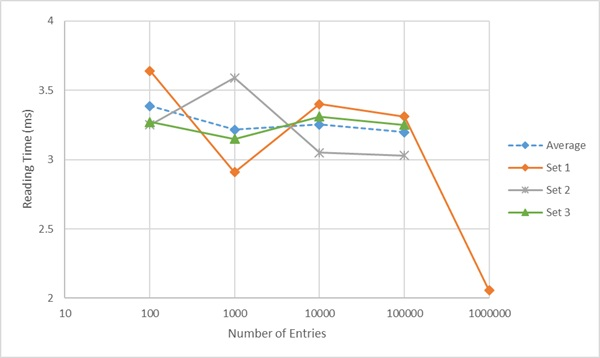
\includegraphics{figures/normalTimes.jpg}
      \caption{Reading Times of 'normal' partitioning schema for different Number of DB Entries. Measruements for a particular Number of entries were performed three times except for 1,000,000 entries, with average displayed.
      \\
      Regression on Average: r=0.56}
      \label{fig:normalTimes}
  \end{figure}
  
  \begin{figure}[H]
      \centering
      \noindent\makebox[\textwidth]{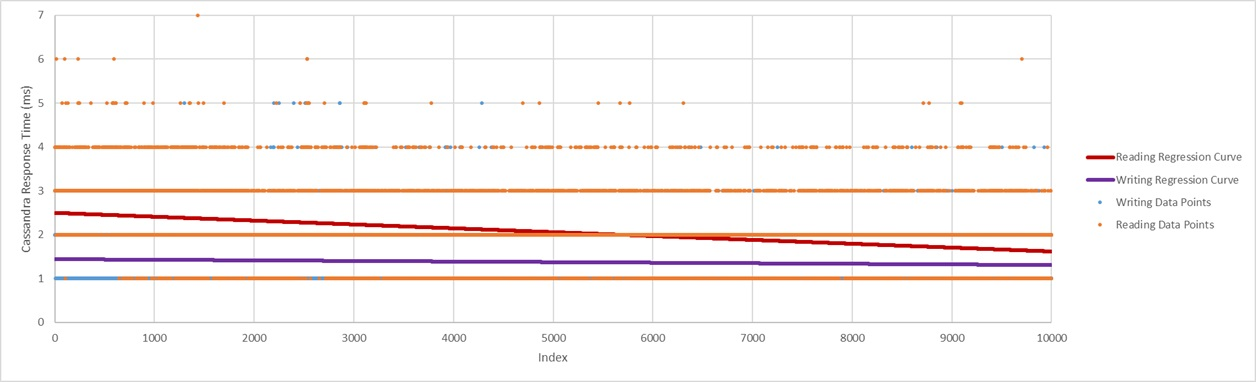
\includegraphics[width=\paperwidth]{figures/normalFull.jpg}}
      \caption{Writing and Reading Times for the 'normal' partitioning schema, at an Entry Number of 1,000,000 and sample size of 10,000. Note that some outliers above 7 ms (approaching 25 ms) were excluded in the chart in favour of more clear display.
      \\
      Regression: r=0.067 for writing and r=0.27 for reading}
      \label{fig:normalFull}
  \end{figure}
  
  \subsection{The 'Worst' Case}
  
  \begin{figure}[H]
      \centering
      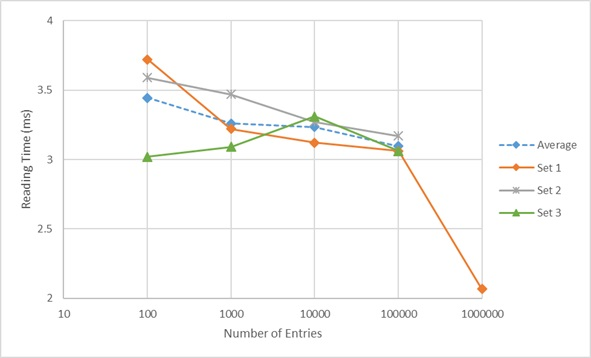
\includegraphics{figures/worstTimes.jpg}
      \caption{Reading Times of 'worst' partitioning schema for different Number of DB Entries. Measruements for a particular Number of entries were performed three times except for 1,000,000 entries, with average displayed.
      \\
      Regression on Average: r=0.79}
      \label{fig:worstTimes}
  \end{figure}
  
  \begin{figure}[H]
      \centering
      \noindent\makebox[\textwidth]{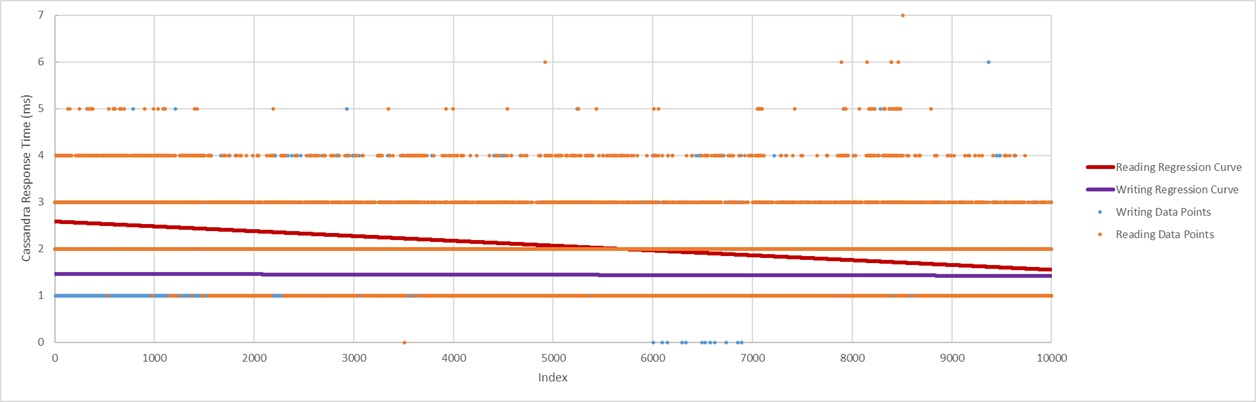
\includegraphics[width=\paperwidth]{figures/worstFull.jpg}}
      \caption{Writing and Reading Times for the 'worst' partitioning schema, at an Entry Number of 1,000,000 and sample size of 10,000. Note that some outliers above 7 ms (approaching 35 ms) were excluded in the chart in favour of more clear display.
      \\
      Regression: r=0.012 for writes and r=0.29 for reading.}
      \label{fig:worstFull}
  \end{figure}
  
  \subsection{Comparing the Cases}
  
  \begin{figure}
      \centering
      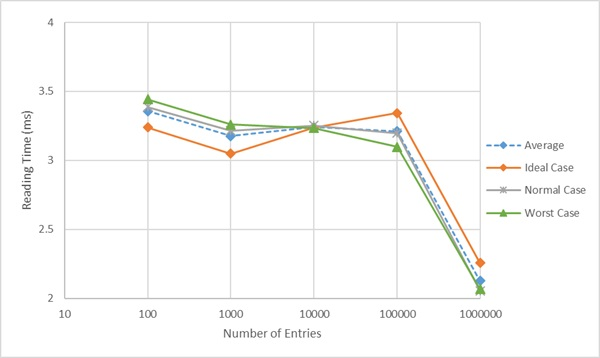
\includegraphics{figures/allTimes.jpg}
      \caption{Comparison of all three partition Schema per Number of Entries with Average. Note how all methods perform exactly equal at 10,000 entries and more importantly the extreme reduction in reading time for all schema at 1,000,000 entries. \\  Regression on Average: r=0.990}
      \label{fig:allTimes}
  \end{figure}
  
  \begin{figure}[H]
      \centering
      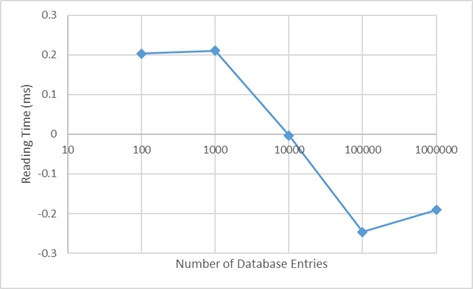
\includegraphics{figures/worstIdealTimes.jpg}
      \caption{Difference in Mean Reading Times for the 'worst' and 'ideal' schema, per Number of DB Entries.
      \\
      Regression: r=0.56}
      \label{fig:worstIdeal}
  \end{figure}
  
  \begin{figure}[H]
      \centering
      \noindent\makebox[\textwidth]{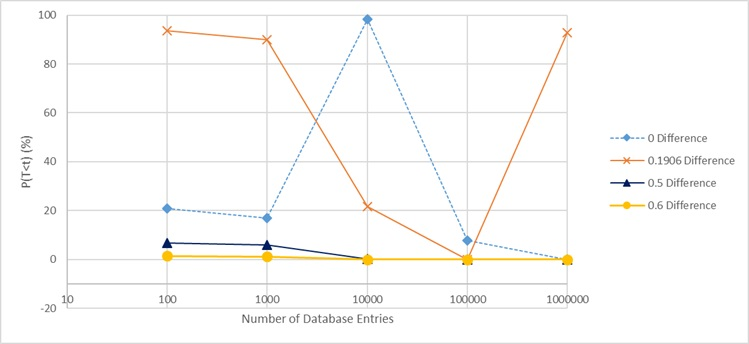
\includegraphics[width=\linewidth]{figures/tTest.jpg}}
      \caption{t-Test Comparison of 'ideal' and 'worst' partitioning Schema showing \(P_{(T<t)}\) in percent.}
      \label{fig:tTest}
  \end{figure}
  
\section{Discussion} % 400 words
\label{sec:discuss}

  The Data shows that, surprisingly, what was expected to be the worst partitioning schema actually performs slightly better at larger Data sets, while perhaps less surprisingly reading times plummet with the number of consecutive reads. 
  
  \subsection{Reading Times per Number of Reads}
  As Figure \ref{fig:allTimes} shows the time that reads require to return Data actually reduces with the number of entries. It should be considered that the independent axis here is logarithmic which perhaps helps explain the comparatively large difference between the last two Data points, as they are almost literally a million 'reads' apart. Regression shows that this reduction is not merely accidental but there is some correlation. 
  \\
  Perhaps some form of predictive execution plays a role in this correlation, in particular as the last Data point has a significantly larger sample size allowing for more adaptation. Figures \ref{fig:idealFull}, \ref{fig:normalFull} and \ref{fig:worstFull} suggest that reading times decrease with the number of reads gradually, though Regression does not support this hypothesis. However, it cannot reject it, and either more precise measurements or even larger experiments could shed some light on this idea. It certainly appears reasonable that Predictive Processing by the CPU would increasingly favour repetitive processes and some reuse of resources might have further effect. Perhaps Cassandra is even progressively assigned more resources as the process continues, allowing it to perform better, and this happens to directly correlate with the length of the experiment.
  
  \subsection{The Effect of Partition Size}
  Originally it was hypothesised that larger partitions would negatively affect reading times as they would require the DB to search through larger Data Sets after localising the correct partition and this was supported by the literature. \cite{ctoAnalysis} However, Figures \ref{fig:allTimes} and \ref{fig:tTest} show that there is a very small but clear difference in favour of larger partitions with what was considered the worst schema and in the end 1,000,000 entries in only one partition outperforms what was considered the ideal schema with only 10 entries for each partition. While this correlation is likely to be statistically significant it is below 0.20 ms and is in this experiment indistinguishable from the difference due to the number of partitions, as here partition size and number of partitions are directly correlated by design. 
  \\
  It is quite possible that larger partitions do not perform significantly different from smaller ones as entries are sorted within Cassandra and were in this experiment not inserted or queried in random order. Perhaps randomising the keys both when populating the DB and when querying would shed more light on this aspect, but for now it is reasonable to presume, without any guarantee, that there might be no difference in performance due to partition size and the Data may be explained entirely by the last factor: the number if partitions in the DB. 
  
  \subsection{Number of Partitions}
  Finally, it would appear that the number of partitions is the most significant factor in explaining the difference in performance between the 'ideal' and 'worst' partitioning schema. As Figure \ref{fig:tTest} shows there is no statistically clear winner between the two before 1,000,000 entries and here the difference is below 0.20 ms. In fact below 10,000 DB entries the 'ideal' schema appears to perform better, though the hypothesis that the two perform equally cannot technically be rejected. From here the 'worst' schema appears to grow slightly faster than the 'ideal' one.
  \\
  It would be beneficial to investigate whether or not this trend continues for larger entry numbers and, of course, how this affects other performance like writes, deletes and updates. Since Cassandra is optimised for writing however, these quantities should not be as severely affected and differences will likely be difficult to investigate. \cite{ctoAnalysis,cassandraBasics,cassandraKey} As larger partitions force more Data into the same SSTables compaction might be affected by the partitioning schema.
  \\
  Another possible direction of research would be the effect of more complex Data Models on this trend. Cassandra and other NoSQL Databases commonly trade in writes for reading efficiency because writes are already so efficient, which can also be observed in Figures \ref{fig:idealFull}, \ref{fig:normalFull} and \ref{fig:worstFull}. This is normally significant with complex Data Models where the same Data must be optimised for several queries which makes duplication at write time more efficient than complex join operations at read time. \cite{cassandraBasics,sherman}
  
  %\subsection{Further Considerations and Suggestions}
  

\section{Conclusion} % 100 words
\label{sec:conc}

  While in a distributed Cassandra Database Cluster good practice is considered to partition Data into many smaller partitions that can be evenly spread throughout the Cluster, this rather small experiment calls this practice into question for applications within just one machine. In fact it is possible that increasing the number of partitions even negatively impacts performance. 
  \\
  While a small effect could be demonstrated for reading operation, other operations are unlikely to be affected equally and further investigation is required to clarify to what extend it might really be advantagous to break common practice in this rather unusual use case.


\clearpage
\bibliography{myrefs}
%\printbibliography

\end{document}
